\section{Ingeniería de requisitos}

\begin{orientacion}
Formule requisitos verificables. Evite expresiones ambiguas como ``rápido'', ``eficiente'' o ``adecuado''. Cada requisito debe tener identificador, descripción, criterio de aceptación, prioridad, fuente y método de verificación.
\end{orientacion}

\subsection{Matriz de requisitos}

\begingroup
\scriptsize
\setlength{\tabcolsep}{3pt}
\renewcommand{\arraystretch}{1.2}

% Anchos de columna como fracción de \textwidth (suman 1.0 = 100%)
\newlength{\colID}
\newlength{\colCat}
\newlength{\colReq}
\newlength{\colCrit}
\newlength{\colPrio}
\newlength{\colVer}

\setlength{\colID}{0.07\textwidth}
\setlength{\colCat}{0.13\textwidth}
\setlength{\colReq}{0.34\textwidth}
\setlength{\colCrit}{0.29\textwidth}
\setlength{\colPrio}{0.07\textwidth}
\setlength{\colVer}{0.10\textwidth}

\begin{longtable}{
  >{\bfseries}p{\colID}
  p{\colCat}
  p{\colReq}
  p{\colCrit}
  p{\colPrio}
  p{\colVer}
}
\caption{Matriz de requisitos del sistema.} \label{tab:matriz_requisitos} \\

\toprule
\textbf{ID} & \textbf{Categoría} & \textbf{Requisito verificable} & \textbf{Criterio de aceptación} & \textbf{Prioridad} & \textbf{Verificación} \\
\midrule
\endfirsthead

\multicolumn{6}{c}{\tablename\ \thetable\ -- continuación} \\
\toprule
\textbf{ID} & \textbf{Categoría} & \textbf{Requisito verificable} & \textbf{Criterio de aceptación} & \textbf{Prioridad} & \textbf{Verificación} \\
\midrule
\endhead

\midrule
\multicolumn{6}{r}{\textit{Continúa en la siguiente página}} \\
\endfoot

\bottomrule
\endlastfoot

REQ-01 & Proceso & El sistema deberá ejecutar de forma automática un ciclo completo de lavado CIP (enjuague inicial, lavado con solución de jabón, enjuague final) sin intervención manual una vez iniciado desde el panel de control. & Ciclo completo ejecutado en la secuencia correcta en 3 pruebas consecutivas, sin intervención del operador. & Alta & Prueba funcional \\[3pt]

REQ-02 & Funcional & El sistema deberá secuenciar automáticamente la apertura y cierre de las tres electroválvulas según la etapa del ciclo (llenado, lavado, enjuague), evitando que dos etapas incompatibles se ejecuten simultáneamente. & Secuencia de electroválvulas ejecutada en el orden correcto sin traslapes, verificada en 3 pruebas consecutivas. & Alta & Prueba funcional \\[3pt]

REQ-03 & Portabilidad & La estructura del sistema, en condición de vacío (sin líquido en los tanques), deberá tener un peso que no exceda el límite de carga manual recomendado para levantamiento ocasional por una persona (referencia NIOSH, aprox. 23 kg), y su chasis deberá soportar sin deformación ni pérdida de estabilidad el peso adicional de los tres tanques llenos. & Peso en vacío medido $\leq$23 kg, y chasis sin deformación visible ni volcamiento con los tres tanques llenos, verificado en prueba de carga estática. & Alta & Prueba \\[3pt]

REQ-04 & Portabilidad & El sistema deberá contar con ruedas y puntos de anclaje/asas que permitan su traslado, nivelación y fijación en un tiempo menor a 10 minutos. & Traslado, nivelación y fijación completados en $\leq$10 min, verificado por cronómetro. & Media & Prueba \\[3pt]

REQ-05 & Hidráulico & El sistema deberá impulsar el fluido de proceso a través de la tubería de acero inoxidable 304 de 1 pulgada (longitud total aproximada de 6 m), garantizando un flujo continuo y suficiente para el arrastre de residuos en todo el recorrido de la tubería, sin zonas muertas ni estancamiento del fluido. & Flujo continuo observado en todo el recorrido de la tubería durante el ciclo completo, sin puntos de estancamiento visibles. & Alta & Prueba \\[3pt]

REQ-06 & Hidráulico & El sistema deberá contar con tres tanques independientes (agua/mezcla $\geq$20 L, jabón $\geq$5 L, agua residual $\geq$20 L) con conexiones herméticas que eviten fugas durante todo el ciclo. & Cero fugas visibles durante prueba de llenado y ciclo completo de 30 min. & Alta & Prueba/ Inspección \\[3pt]

REQ-07 & Eléctrico & La bomba principal AC deberá protegerse mediante un contactor y un relé térmico de sobrecarga dimensionados según la corriente nominal del motor ($\pm$10\%). & Contactor y relé térmico seleccionados verificados contra placa de datos del motor. & Alta & Inspección \\[3pt]

REQ-08 & Eléctrico & El sistema deberá alimentarse con energía monofásica 110/220 VAC y contar con protección contra sobrecorriente y falla a tierra (breaker/diferencial) en el tablero de control. & Disparo del breaker/diferencial verificado ante falla simulada de sobrecorriente o fuga a tierra. & Alta & Prueba \\[3pt]

REQ-09 & Electrónico & La bomba dosificadora peristáltica de 12 VDC deberá controlarse mediante salida a relé del PLC (encendido/apagado temporizado, sin PWM), permitiendo dosis configurables por tiempo de activación. & Volumen dosificado repetible con variación $\leq$10\% entre 3 pruebas para un mismo tiempo de activación. & Alta & Prueba \\[3pt]

REQ-10 & Electrónico & El sistema deberá contar con una fuente de alimentación regulada de 24 VDC para sensores y electrónica de campo, con capacidad de corriente suficiente para todos los consumos (+30\% de margen) y regulación $\leq$5\%. & Voltaje de salida medido dentro de $\pm$5\% bajo carga máxima estimada. & Media & Prueba \\[3pt]

REQ-11 & Instrumentación & El sistema deberá medir el nivel de líquido en el tanque de agua/mezcla mediante un sensor de nivel (flotador o ultrasónico) con una precisión de $\pm$5\% del rango medido. & Lectura de nivel validada contra medición manual (regla/marca) con error $\leq$5\%. & Alta & Prueba \\[3pt]

REQ-12 & Instrumentación & El sistema deberá medir la temperatura del fluido de proceso mediante un sensor (tipo PT100, termopar o DS18B20) en un rango de 0-80 °C con precisión de $\pm$1 °C. & Lectura del sensor comparada contra termómetro patrón con error $\leq$1 °C en todo el rango de operación. & Alta & Prueba \\[3pt]

REQ-13 & Control & El PLC (S7-1200 CPU 1214C) deberá ejecutar un lazo de control que mantenga la temperatura del fluido dentro del rango de 40-50 °C con un error en estado estable $\leq$2 °C. & Temperatura estabilizada dentro de 40-50 °C $\pm$2 °C durante al menos 5 min continuos. & Alta & Prueba \\[3pt]

REQ-14 & Control & El sistema deberá detener automáticamente el elemento de calentamiento y activar una alarma si la temperatura del fluido supera el umbral de seguridad de 60 °C. & Corte del calentador verificado  al superar 60 °C en prueba controlada. & Alta & Prueba \\[3pt]

REQ-15 & Comunicaciones Industriales & El PLC deberá comunicarse mediante Ethernet/PROFINET con la interfaz HMI local, permitiendo el monitoreo y control en tiempo real de nivel, temperatura y estado del ciclo. & Datos de proceso visibles y actualizados en HMI . & Media & Prueba \\[3pt]

REQ-16 & Supervisión IoT & El sistema deberá enviar periódicamente ($\leq$30 s) los datos de temperatura, nivel y estado del ciclo a una plataforma de supervisión remota mediante un gateway IoT (p. ej. ESP32/Node-RED). & Datos recibidos en la plataforma remota con periodo $\leq$30 s durante prueba de 15 min. & Media & Prueba \\[3pt]

REQ-17 & Supervisión IoT & El sistema deberá permitir la visualización remota del estado del ciclo (en curso, finalizado, alarma) desde un dispositivo móvil o PC conectado por WiFi/Ethernet. & Estado del ciclo correctamente reflejado en el dispositivo remoto en las 3 condiciones evaluadas. & Media & Prueba \\[3pt]

REQ-18 & Seguridad & El sistema deberá contar con un paro de emergencia (tipo hongo) que interrumpa la alimentación de los actuadores principales (bomba, calentador, dosificador) en menos de 1 segundo al activarse. & Corte de energía a actuadores principales verificado en $\leq$1 s tras accionar el paro de emergencia. & Alta & Prueba \\[3pt]

REQ-19 & Seguridad & El sistema deberá activar una alarma visual y sonora ante condiciones anómalas (nivel bajo, sobretemperatura, falla de bomba) detectadas por los sensores del sistema. & Alarma visual y sonora activada correctamente ante cada una de las 3 condiciones simuladas. & Alta & Prueba \\[3pt]

REQ-20 & Documentación/ Validación & El proyecto deberá entregar manual de usuario, planos eléctricos e hidráulicos, y un protocolo de pruebas de validación, en formato digital editable y PDF. & Documentos entregados completos, revisados y aprobados por el equipo antes de la entrega final. & Media & Inspección \\

\end{longtable}
\endgroup

La matriz de requisitos permite establecer de manera organizada las condiciones que debe cumplir el sistema CIP. Los requisitos se clasifican de acuerdo con las diferentes áreas involucradas en el diseño, construcción, operación y validación del sistema.

Se consideran requisitos funcionales y de proceso, mecánicos y de portabilidad, hidráulicos, eléctricos, electrónicos, de instrumentación, control, comunicaciones, supervisión mediante IoT, seguridad, documentación y validación.

\subsection{Despliegue de la función de calidad -- QFD}

\begin{orientacion}
Relacione necesidades del usuario con características técnicas. Use la sigla QFD, correspondiente a \textit{Quality Function Deployment}. Incorpore la matriz completa como figura legible o anexo y resuma aquí sus resultados.
\end{orientacion}

\begin{figure}[H]
    \centering
    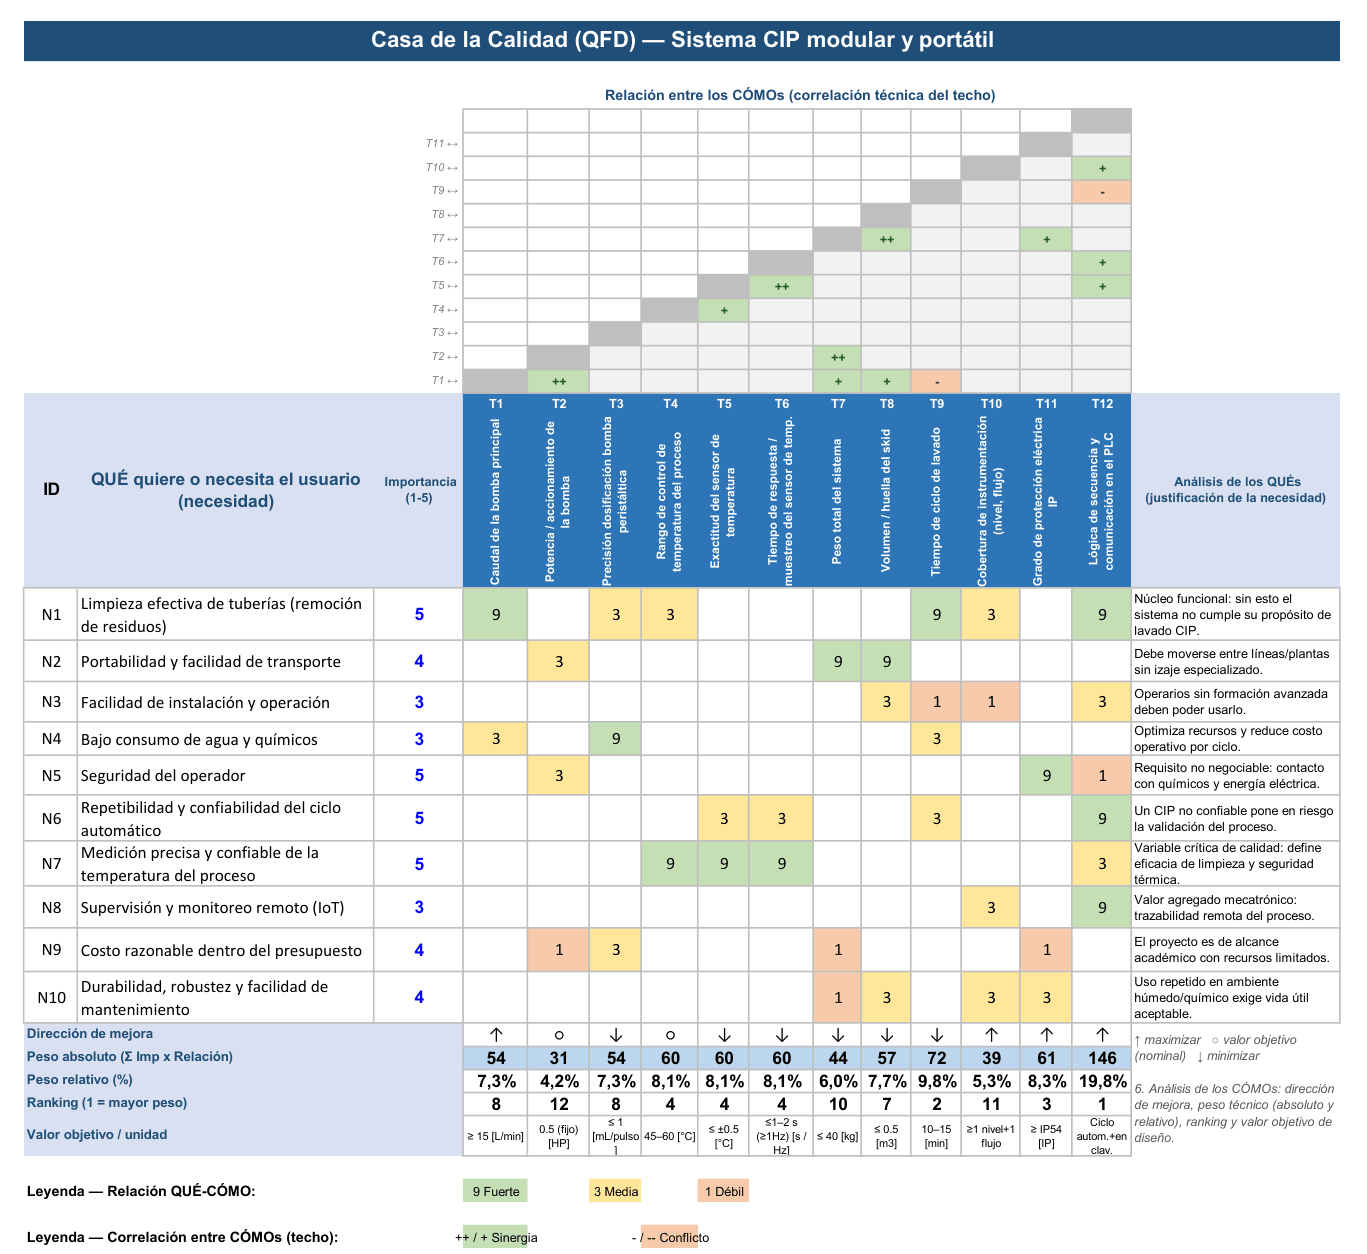
\includegraphics[width=\textwidth]{figuras/matriz_qfd.png}
    \caption{Matriz QFD del sistema CIP.}
    \label{fig:qfd}
\end{figure}

\campo{Analice las características técnicas con mayor ponderación y su influencia sobre el diseño.}

La matriz QFD permite relacionar las necesidades identificadas por los usuarios con las características técnicas del sistema CIP. A partir de esta relación se pueden establecer las características de diseño que tienen mayor influencia sobre el desempeño del sistema.

Las características técnicas con mayor ponderación deben recibir una atención prioritaria durante las etapas de diseño e implementación, debido a que tienen una mayor influencia sobre el cumplimiento de las necesidades del usuario. Esta priorización permite orientar la selección de componentes, la arquitectura del sistema, los elementos de instrumentación, los actuadores y las estrategias de control.

Además, el QFD facilita la toma de decisiones técnicas al establecer una relación entre los requerimientos del usuario y las variables que pueden ser controladas directamente durante el desarrollo del sistema.

\subsection{Matrices de decisión Pugh}

\begin{table}[H]\centering\small\caption{Plantilla de matriz de decisión Pugh.}
\begin{tabularx}{\textwidth}{YL{1.8cm}C{2cm}C{2cm}C{2cm}}\toprule
\textbf{Criterio}&\textbf{Peso}&\textbf{Alternativa A}&\textbf{Alternativa B}&\textbf{Alternativa C}\\\midrule
Compatibilidad&\campo{0--1}&\campo{Puntaje}&\campo{Puntaje}&\campo{Puntaje}\\
Seguridad&\campo{0--1}&\campo{Puntaje}&\campo{Puntaje}&\campo{Puntaje}\\
Costo y disponibilidad&\campo{0--1}&\campo{Puntaje}&\campo{Puntaje}&\campo{Puntaje}\\
Mantenibilidad&\campo{0--1}&\campo{Puntaje}&\campo{Puntaje}&\campo{Puntaje}\\\midrule
\textbf{Total ponderado}&1.00&\campo{--}&\campo{--}&\campo{--}\\\bottomrule
\end{tabularx}\end{table}


\campo{Repita la matriz para arquitectura, sensores, actuadores, calentamiento, bomba, válvulas, protocolo y plataforma de supervisión. Explique la ponderación y la alternativa seleccionada.}

Las matrices de decisión Pugh permiten comparar diferentes alternativas de diseño utilizando criterios previamente establecidos. Para cada alternativa se asigna una valoración con respecto a una referencia, permitiendo identificar aquella que presenta el mejor comportamiento global frente a los requisitos definidos.

La ponderación de los criterios debe considerar su importancia dentro del funcionamiento del sistema CIP. Entre los aspectos que pueden evaluarse se encuentran el cumplimiento funcional, costo, facilidad de implementación, disponibilidad de los componentes, mantenimiento, seguridad, compatibilidad con el sistema y posibilidad de integración con los demás elementos.

Este procedimiento se aplica a la selección de la arquitectura del sistema, sensores, actuadores, sistema de calentamiento, bomba, válvulas, protocolo de comunicación y plataforma de supervisión. La alternativa seleccionada será aquella que obtenga la mejor valoración global y que, además, cumpla con los requisitos establecidos para el sistema.